\part{Implémentation}

\section{Structure du programme}
Nous avons implémenté nos algorithmes en java en utilisant la bibliothèque jgrapht pour la gestion des graphes. Voici la structure générale du programme :\newline

\scalebox{0.7} {
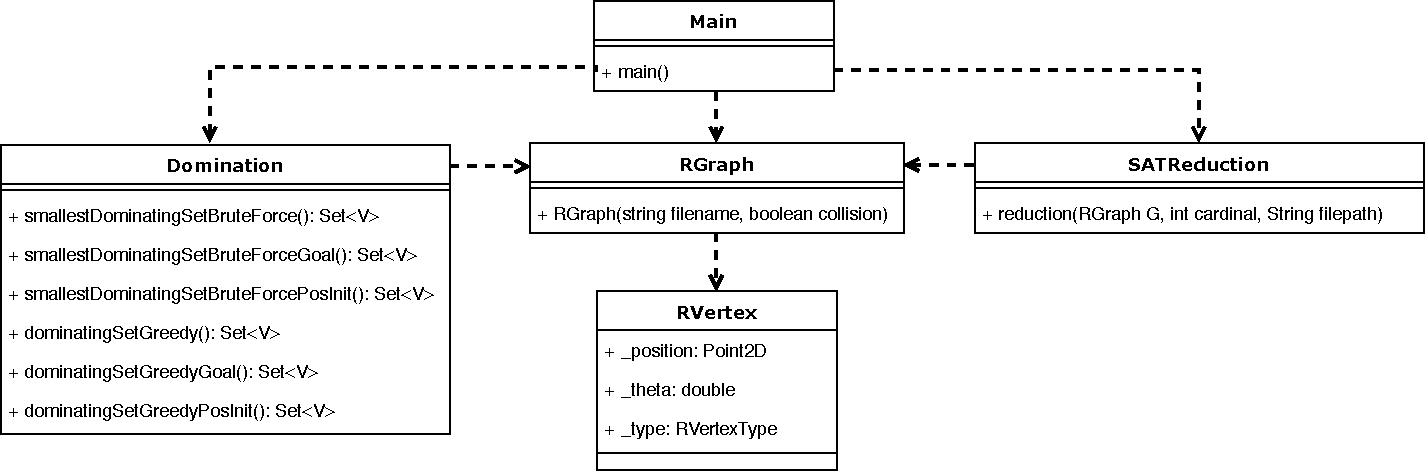
\includegraphics{robotdef.pdf}
} \newline

Le constructeur de la classe RGraph est capable de lire un fichier d'entrée json pour créer un graphe modélisant le problème correspondant. Les sommets de RGraph sont des RVertex. Un RVertex est composé d'une position, d'un angle de tir si le sommet est un sommet de tir et d'un type qui décrit si le sommet est un sommet de tir ou de position (ou un sommet de position surface de réparation dans le cas de l'extension goal). La classe Domination contient les implémentations des algorithmes de résolution et la classe SATReduction la réduction vers SAT. La fonction reduction sauvegarde la formule SAT dans un fichier en format dimacs. Notre programme peut ensuite demander au solveur SAT glucose de tester la satisfaisabilité de cette formule.

\section{Utilisation}

À COMPLÉTER

\section{Résultats}

À COMPLÉTER